\documentclass{article}
\usepackage{spconf,amsmath,amsfonts,amssymb}
\interdisplaylinepenalty=2500

%% Accents Français pour le nom de l'école
\usepackage[utf8]{inputenc}
\usepackage[usenames,dvipsnames]{color}
\usepackage{pifont} % pour certains dingbats
\usepackage[normalem]{ulem} % pour strike
\usepackage{setspace} % pour spacing
\usepackage{graphicx}
\usepackage{hyperref}
% http://en.wikibooks.org/wiki/LaTeX/Hyperlinks
\hypersetup{
    colorlinks=true,    % false: boxed links; true: colored links
    linkcolor=blue,    % color of internal links
    citecolor=blue,    % color of links to bibliography
    filecolor=blue,    % color of file links
    urlcolor=blue      % color of external links
}

\newcommand{\ltCodec}{H.264/AVC JM reference software}

% petite macro pour marquer les points
% a completer.
\newcommand{\fillme}[1]{\ding{118}}
%\renewcommand{\sout}[1]{} % uncomment to hide \sout text


\title{Pixel Domain Referenceless Visual Degradation Detection\\
and Error Concealment for Mobile Video}

%% sneaky baseline stretch
\renewcommand{\baselinestretch}{0.925}
%DIF PREAMBLE EXTENSION ADDED BY LATEXDIFF
%DIF UNDERLINE PREAMBLE %DIF PREAMBLE
\RequirePackage[normalem]{ulem} %DIF PREAMBLE
\RequirePackage{color}\definecolor{RED}{rgb}{1,0,0}\definecolor{BLUE}{rgb}{0,0,1} %DIF PREAMBLE
\providecommand{\DIFaddtex}[1]{{\protect\color{blue}\uwave{#1}}} %DIF PREAMBLE
\providecommand{\DIFdeltex}[1]{{\protect\color{red}\sout{#1}}}                      %DIF PREAMBLE
%DIF SAFE PREAMBLE %DIF PREAMBLE
\providecommand{\DIFaddbegin}{} %DIF PREAMBLE
\providecommand{\DIFaddend}{} %DIF PREAMBLE
\providecommand{\DIFdelbegin}{} %DIF PREAMBLE
\providecommand{\DIFdelend}{} %DIF PREAMBLE
%DIF FLOATSAFE PREAMBLE %DIF PREAMBLE
\providecommand{\DIFaddFL}[1]{\DIFadd{#1}} %DIF PREAMBLE
\providecommand{\DIFdelFL}[1]{\DIFdel{#1}} %DIF PREAMBLE
\providecommand{\DIFaddbeginFL}{} %DIF PREAMBLE
\providecommand{\DIFaddendFL}{} %DIF PREAMBLE
\providecommand{\DIFdelbeginFL}{} %DIF PREAMBLE
\providecommand{\DIFdelendFL}{} %DIF PREAMBLE
%DIF END PREAMBLE EXTENSION ADDED BY LATEXDIFF
%DIF PREAMBLE EXTENSION ADDED BY LATEXDIFF
%DIF HYPERREF PREAMBLE %DIF PREAMBLE
\providecommand{\DIFadd}[1]{\texorpdfstring{\DIFaddtex{#1}}{#1}} %DIF PREAMBLE
\providecommand{\DIFdel}[1]{\texorpdfstring{\DIFdeltex{#1}}{}} %DIF PREAMBLE
%DIF END PREAMBLE EXTENSION ADDED BY LATEXDIFF

\begin{document}

% allow more graphics in a page/column
\renewcommand{\topfraction}{0.9}
\DIFdelbegin %DIFDELCMD < \renewcommand{\bottomfraction}{0.5}
%DIFDELCMD < 

%DIFDELCMD < \renewcommand{\textfraction}{0.05}
%DIFDELCMD < %%%
\DIFdelend \DIFaddbegin \renewcommand{\textfraction}{0.1}
\DIFaddend \renewcommand{\floatpagefraction}{0.9}

%% sets only one space after .
\frenchspacing
%% less space after/before figures
\DIFdelbegin %DIFDELCMD < \setlength{\textfloatsep}{0.5em}
%DIFDELCMD < %%%
\DIFdelend \DIFaddbegin \setlength{\textfloatsep}{1em}
\DIFaddend 

%DIF < \setlength{\abovedisplayskip}{0.75em}
%DIF < \setlength{\belowdisplayskip}{0.75em}
%DIF < \setlength{\parskip}{1em plus 1em minus 0.5 em}
\DIFaddbegin \setlength{\abovedisplayskip}{0.75em}
\setlength{\belowdisplayskip}{0.75em}
\setlength{\parskip}{0em}
\DIFaddend 





\name{Luc Trudeau, Stéphane Coulombe, Steven Pigeon\thanks{\scriptsize This
work was supported in part by the Natural Sciences and Engineering Research
Council of Canada under research grant \#356807-07, and in part by
\textit{Le Fonds québécois de la recherche sur la nature et les
technologies} (FQRNT) under research grant \#141698. Emails:
luc.trudeau.1@ens.etsmtl.ca, \{stephane.coulombe,
steven.pigeon\}@etsmtl.ca}} \address{Department of Software and IT
Engineering\\ École de technologie supérieure, Université du
Québec\\ Montréal, Québec, Canada}

\maketitle


%%%%%%%%%%%%%%%%%%%%%%%%%%%%%%%%% ABSTRACT %%%%%%%%%%%%%%%%%%%%%%%%%%%%%%%%%
\begin{spacing}{0.9}
\begin{abstract}
\small In mobile video applications, where unreliable networks are
commonplace, corrupted video packets can have a profound impact on the
quality of the user experience. In this paper, we \DIFaddbegin \DIFadd{will }\DIFaddend show that, in a wide
range of operating conditions, selectively reusing data resulting from
decodable \DIFdelbegin \DIFdel{errorneous }\DIFdelend \DIFaddbegin \DIFadd{broken }\DIFaddend packets leads to better results than frame copy. This
selection is guided by a novel concept that combines motion estimation
and a measure of blocking artifacts at block edges to predict visual
degradation caused by the decoding of erroneous packets. Simulation results
show that, by using the proposed solution, the \ltCodec{} decoder can
select the best option between frame copy and the erroneous frame decoding in
82\% of \DIFaddbegin \DIFadd{the }\DIFaddend test cases. We also obtain an average gain of 1.95\DIFaddbegin \DIFadd{~}\DIFaddend dB
for concealed frames \DIFdelbegin \DIFdel{(when they }\DIFdelend \DIFaddbegin \DIFadd{that }\DIFaddend differ from those concealed by the JM decoder\DIFdelbegin \DIFdel{)}\DIFdelend .
\end{abstract}

\begin{keywords}
\small Error concealment, error detection, H.264, mobile video, pixel domain
\end{keywords}
\end{spacing}


%%%%%%%%%%%%%%%%%%%%%%%%%%%%%%%%% INTRO %%%%%%%%%%%%%%%%%%%%%%%%%%%%%%%%%
\DIFaddbegin \vspace{-0.5em}\DIFaddend \begin{section}{Introduction}
\label{section-introduction}
The capabilities of modern video coding standards like H.264 have paved the
way for new consumer market video applications, such as video conferencing,
video telephony, and video streaming over wireless networks using mobile
devices. Operating conditions in wireless networks are far from ideal for
video applications. These network media are unreliable and data loss is
unavoidable, which increases the complexity of video-based applications
that must recover from the error either by retransmission or by
concealment. These limitations must be addressed to ensure the success of
wireless video applications.

The impracticality of retransmission in live video makes error
concealment the preferred method of error recovery~\cite{Wang1998}. Error
concealment approaches were developed to improve the perceived quality of
decoded sequences that have been subject to packet corruption over
unreliable networks. However, error concealment algorithms will either
conceal the whole slice~\cite{Wu-ISCAS-2006}, or perform block-level
concealment~\cite{OBMA}. The latter requires knowledge of erroneous blocks
in the corrupted frame~\cite{Wang1998}.

In H.264, slices are independently decodable groups of blocks. When an erroneous
packet is discarded at the network level, the corresponding slice is lost, even
if the blocks preceding the error are valid or if the visual impairment
resulting from the error is minor. However, in the context of mobile
applications, where bit rates are low and resolutions small, dropping a packet
entails losing critical parts of a frame, and in some cases the entire frame.
Even with state-of-the-art error concealment approaches, this \DIFdelbegin \DIFdel{may }\DIFdelend leads to 
significant visual degradation\DIFaddbegin \DIFadd{, }\DIFaddend which will propagate in subsequent frames.

In~\cite{Superiori2007}, Superiori \textit{et al.} have shown that using
information from \DIFdelbegin \DIFdel{\emph{decodable} (i.e. decoding them will not crash the 
decoder)
}\DIFdelend \DIFaddbegin \DIFadd{decodable }\DIFaddend erroneous packets can yield beneficial results.
However, reusing erroneous packets can lead to the following artifacts:
spatially shifted blocks, inverse DCT related noise, empty blocks (green or
black), or frame freeze, the effects of which depend on the decoder used.

In cases where corrupted bit streams are decodable, the information they
contain, even if it is damaged, once analyzed by the proposed detection approach,
could be beneficial in guiding decisions made by a concealment module for either 
a whole slice concealment method (currently what is avaible in the \ltCodec{} decoder, 
and will be presented in this work) or for a block level concealment approach 
such as the recent findings on outer boundary matching algorithms ~\cite{OBMA}.
\DIFdelbegin \DIFdel{The term ``slice concealment'' describes a family of concealment algorithms 
that conceal the whole slice, such as frame copy and motion 
copy~}%DIFDELCMD < \cite{Wu-ISCAS-2006}%%%
\DIFdel{.
}\DIFdelend 

This paper is organized as follows. \DIFdelbegin \DIFdel{In 
}\DIFdelend \DIFaddbegin \DIFadd{First, in 
}\DIFaddend section~\ref{section-motion-compensated-blockiness}, we propose a solution,
based on the novel concept of motion-compensated blockiness, to identify
visually degraded regions in predicted \DIFdelbegin \DIFdel{(P) }\DIFdelend frames caused by damaged, but decodable,
packets. The proposed detection process is intended for block-based \DIFaddbegin \DIFadd{DCT }\DIFaddend codecs.
It operates in the pixel domain and is independent of decoder-specific
information, such as block size or bitrate. 
Section~\ref{section-selective-slice-concealment} presents the
concept of selective slice concealment, a low-complexity add-on to modern
decoders where motion-compensated blockiness is used to perform referenceless
visual degradation detection to guide the choice between using a slice
concealment candidate or the erroneous slice when \DIFdelbegin \DIFdel{concealing }\DIFdelend \DIFaddbegin \DIFadd{rebuilding }\DIFaddend a corrupted frame.
In section~\ref{section-experimental-results}, we present the experimental 
results of our proposed error detection and concealment solution using H.264, 
and we present our conclusions in section~\ref{section-conclusion}.
\end{section}
%%%%%%%%%%%%%%%%%%%%%%%%%%%%%%%%% MOTION COMPENSATED BLOCKINESS
%%%%%%%%%%%%%%%%%%%%%%%%%%%%%%%%%
\newcommand{\ltSlice}[1]{\mathbf{S}_{#1}}
\newcommand{\ltF}[1]{\mathbf{F}_{#1}}
\newcommand{\ltP}[1]{\mathbf{P}_{#1}}
\newcommand{\ltD}[1]{\mathbf{D}_{#1}}
\newcommand{\ltI}[1]{\mathbf{I}_{#1}}
\newcommand{\ltR}[1]{\mathbf{R}_{#1}}
\newcommand{\ltB}[1]{\mathbf{B}_{#1}}
\newcommand{\ltS}[1]{\mathcal{I}_{#1}}
\newcommand{\ltErr}[1]{\mathbf{\hat{F}}_{#1}}
\newcommand{\ltConc}[1]{\mathbf{F^{\prime}}_{#1}}
\newcommand{\ltOpt}[1]{\mathbf{F^{*}}_{#1}}

\newcommand{\ltMIN}[1]{\arg \min_{#1}}

\newcommand{\ltCB}[2]{\mathbf{b}_{#1}(#2)}
\newcommand{\ltBor}[1]{\mathcal{#1}}
\newcommand{\lttBLK}[2]{\textrm{MCB}_{#1}(#2)}
\newcommand{\ltSTBLK}[1]{\textrm{SMCB}(#1)}
\newcommand{\ltBV}[1]{\mathbf{BV}_{#1}}

\newcommand{\ltSAD}[1]{\textrm{SAD}(#1)} 

\DIFaddbegin \vspace{-0.5em}\DIFaddend \begin{section}{Motion-Compensated Blockiness}
\label{section-motion-compensated-blockiness} % if ever needed
It is a known fact that a corrupted bit stream \DIFdelbegin \DIFdel{can }\DIFdelend \DIFaddbegin \DIFadd{will }\DIFaddend desynchronize a decoder. 
This will often break the spatial pixel correlation in frame content at the 
block boundaries. Blockiness, a measure of \DIFdelbegin \DIFdel{the visibility of blocking artifacts}\DIFdelend \DIFaddbegin \DIFadd{blocking artifact visibility}\DIFaddend , is a
predominant feature of \DIFdelbegin \DIFdel{the }\DIFdelend visual impairment caused by decoder
desynchronization~\cite{Superiori2007}. In~\cite{Superiori2007} 
and~\cite{Ikuno2007}, the authors present a no-reference
visual impairment detection method based on 
\begin{equation*}
\label{eq-FrameSub}
\ltD{} = | \ltF{} - \ltP{} |\:,
\end{equation*}
\DIFaddbegin \DIFadd{where $\ltD{}$ is }\DIFaddend the absolute frame difference \DIFdelbegin \DIFdel{, }\DIFdelend computed pixel by pixel 
\DIFdelbegin \DIFdel{\mbox{$\left(\textrm{i.e.~} \ltD{x,y}\!=\!\left| \ltF{x,y} - \ltP{x,y} 
\right|\right)$}, 
}\DIFdelend \DIFaddbegin \DIFadd{$\left(\textrm{i.e.~} \ltD{x,y} = \left| \ltF{x,y} - \ltP{x,y} \right|\right)$ 
}\DIFaddend between the current frame $\ltF{}$ and the previous frame $\ltP{}$, 
assuming that the previous frame is error-free.

To identify \DIFdelbegin \DIFdel{visual }\DIFdelend \DIFaddbegin \DIFadd{image }\DIFaddend degradation caused by decoder desynchronization, Ikuno
\textit{et al.}~\cite{Ikuno2007} measure the block energy and blockiness found 
in frame $\ltD{}$. Values exceeding a certain threshold are considered
erroneous. These results \DIFdelbegin \DIFdel{are }\DIFdelend \DIFaddbegin \DIFadd{have been }\DIFaddend refined with more sophisticated follow-up
techniques, such as voting~\cite{Superiori2007,Ikuno2007} or \DIFdelbegin \DIFdel{support vector
machines}\DIFdelend \DIFaddbegin \DIFadd{a support vector
machine}\DIFaddend ~\cite{Farrugia2008}.

These refinements are required because $\ltD{}$ is not a reliable source of
error detection, as it will falsely detect energy originating from changes 
between $\ltF{}$ and $\ltP{}$, or blockiness inherent in the content of 
$\ltF{}$ that occurs at block boundaries. \DIFdelbegin \DIFdel{Thus, we }\DIFdelend \DIFaddbegin \DIFadd{We }\DIFaddend propose a novel approach in
which the absolute difference is replaced with the motion-compensated
residual absolute difference.

Let $B\times{}B$ be the block size, 
$H$ and $W$ the height and width of the 
frame respectively, with intervals \DIFdelbegin \DIFdel{\mbox{$\ltS{m}\!=\![0,\frac{W}{B}-1]$}
and \mbox{$\ltS{n}\!=\![0,\frac{H}{B}-1]$}}\DIFdelend \DIFaddbegin \DIFadd{$\ltS{m}=[0,\frac{W}{B}-1]$
and $\ltS{n}=[0,\frac{H}{B}-1]$}\DIFaddend , and $p$ 
the half-width of the motion search area. The
optimal vector for motion \DIFdelbegin \DIFdel{estimation, between $\ltF{}$ and $\ltP{}$ }\DIFdelend \DIFaddbegin \DIFadd{compensation }\DIFaddend for a block at block coordinates ($m,n$)
is given by 
\begin{multline}
\label{eq-Vectors}
(\mathbf{U}_{m,n}, \mathbf{V}_{m,n}) = \DIFdelbegin %DIFDELCMD < \ltMIN{(u,v) \in K} %%%
\DIFdel{~ }%DIFDELCMD < \ltSAD{\ltF{}, 
%DIFDELCMD < \ltP{}, mB, nB, u, v} %%%
\DIFdelend \DIFaddbegin \ltMIN{(u,v) \in W} \DIFadd{~ }\ltSAD{mB, nB, u,
v} \DIFaddend \:,
\end{multline} where \DIFdelbegin \DIFdel{$K = [-p,p] \times [-p, p]$}\DIFdelend \DIFaddbegin \DIFadd{$W = [-p,p] \times [-p, p]$}\DIFaddend ,  $m \in \ltS{m}$, $n \in
\ltS{n}$ and
\begin{equation*}
\DIFdelbegin %DIFDELCMD < \ltSAD{\ltF{}, \ltP{}, x,y,u,v} %%%
\DIFdelend \DIFaddbegin \ltSAD{x,y,u,v} \DIFaddend = \sum_{q=0}^{B-1}\sum_{r=0}^{B-1} \left| \ltF{x+q,y+r} -
\ltP{x+q+u,y+r+v} \right|
\DIFdelbegin %DIFDELCMD < \:%%%
\DIFdel{.
}\DIFdelend \end{equation*}

$\mathbf{U}_{}$ and $\mathbf{V}_{}$ are matrices of motion \DIFdelbegin \DIFdel{vector components 
(horizontal and vertical respectively) }\DIFdelend \DIFaddbegin \DIFadd{vectors }\DIFaddend resulting
from the motion search of each block of a frame. \DIFdelbegin \DIFdel{Considering motion can 
significantly
reduce false error }\DIFdelend \DIFaddbegin \DIFadd{The motion search significantly
reduces false }\DIFaddend detection by compensating for motion between $\ltF{}$ and
$\ltP{}$.
\DIFaddbegin 

\DIFaddend However, motion compensation will not detect errors related to content contained
in \DIFdelbegin \DIFdel{both the current and the previous frames
}\DIFdelend \DIFaddbegin \DIFadd{the previous frame }\DIFaddend (e.g. corrupted motion vectors yield blocks in $\ltF{}$
that are contained in $\ltP{}$, yet often exhibit strong blocking artifacts). 
To detect these errors \DIFaddbegin \DIFadd{while remaining insensitive to motion between $\ltF{}$ 
and $\ltP{}$}\DIFaddend , we measure the blockiness \DIFdelbegin \DIFdel{of residual blocks resulting 
from 
motion estimation}\DIFdelend \DIFaddbegin \DIFadd{around each block boundary of the
difference between a block and its motion-estimated counterpart}\DIFaddend . We refer to this
measure as motion-compensated blockiness \DIFdelbegin \DIFdel{~(MCB}\DIFdelend \DIFaddbegin \DIFadd{($\textrm{MCB}$}\DIFaddend ) and define it\DIFaddbegin \DIFadd{,
for each boundary $d \in \mathcal{B}$, with $\mathcal{B}=\{\ltBor{N}, \ltBor{E},
\ltBor{S}, \ltBor{W}\}$, }\DIFaddend as
\begin{multline*}
\lttBLK{d}{\ltF{},\ltP{}, m,n} = \\ \sum_{l = 0}^{B-1} | \ltCB{d,l}{\ltF{},m B,n
B} - \ltCB{d, l}{\ltP{},m B+\mathbf{U}_{m, n}, n B +\mathbf{V}_{m, n}} |
\DIFdelbegin %DIFDELCMD < \:%%%
\DIFdel{,
}\DIFdelend \end{multline*}
\noindent{}\DIFdelbegin \DIFdel{for each boundary $d \in \mathcal{B}$, with \mbox{$\mathcal{B}\!=\!\{\ltBor{N}, \ltBor{E}, \ltBor{S}, \ltBor{W}\}$} and
}\DIFdelend \DIFaddbegin \DIFadd{with }\DIFaddend \mbox{$m \in \ltS{m}$}, \mbox{$n \in \ltS{n}$}\DIFdelbegin \DIFdel{. }\DIFdelend \DIFaddbegin \DIFadd{, and }\DIFaddend $\mathbf{U}$
and $\mathbf{V}$ \DIFdelbegin \DIFdel{are }\DIFdelend given by eq.~\eqref{eq-Vectors}. The blockiness vectors
$\mathbf{b}_{d, l}$ of all four block boundaries are as follows:
\begin{align*}
\ltCB{\ltBor{N}, l}{\ltF{}, x,y} &= \ltF{x+l,y} - \ltF{x+l,y-1}\:, \\
\ltCB{\ltBor{E}, l}{\ltF{}, x,y} &= \ltF{x+B,y+l} - \ltF{x+B-1,y+l}\:, \\
\ltCB{\ltBor{S}, l}{\ltF{}, x,y} &= \ltF{x+l,y+B} - \ltF{x+l,y+B-1}\:, \\
\ltCB{\ltBor{W}, l}{\ltF{}, x,y} &= \ltF{x,y+l} - \ltF{x-1,y+l}\:,
\end{align*}
with $l \in [0, B-1]$, and where $(x,y)$ are the pixel coordinates of the block.
Note that this measure is different than what is proposed in~\cite{OBMA}\DIFdelbegin \DIFdel{, where
only external borders are being matched}\DIFdelend .

The sum of motion-compensated blockiness ($\textrm{SMCB}$) of a block \DIFdelbegin \DIFdel{, }\DIFdelend at block
coordinates $(m,n)$ along its borders $d \in \mathcal{B}$ \DIFdelbegin \DIFdel{, }\DIFdelend is given by
\begin{equation*}
\label{eq-SumTB}
\ltSTBLK{\ltF{},\ltP{}, m,n} =
\sum_{d\:\in\:\mathcal{B}}\lttBLK{d}{\ltF{},\ltP{},m,n}
\DIFdelbegin %DIFDELCMD < \:%%%
\DIFdel{.
}\DIFdelend \end{equation*}

There remains one significant source of false detection when measuring 
$\textrm{MCB}$: blocking artifacts are accounted for in the two blocks that
share a blocky edge. To address this issue, we propose a blockiness distribution
algorithm which assigns the $\textrm{MCB}_d$ of each block boundary to the
adjacent block with the highest $\textrm{SMCB}$.

The blockiness distribution algorithm is applied, in decreasing order of
$\ltSTBLK{\ltF{},\ltP{},m,n}$, to all blocks with \DIFdelbegin \DIFdel{\mbox{$\ltSTBLK{\ltF{},\ltP{},m,n} 
\!\geqslant\!T_b$}}\DIFdelend \DIFaddbegin \DIFadd{$\ltSTBLK{\ltF{},\ltP{},m,n} \geqslant T_b$}\DIFaddend , where $T_b$
is the threshold that determines whether or not an edge is considered blocky. 
\DIFdelbegin \DIFdel{This threshold is further discussed in 
section~\ref{section-experimental-results}.
}\DIFdelend At the end of the process, the motion-compensated blockiness,
$\textrm{MCB}$, of each blocky edge is assigned to a single block. This yields 
$\textrm{SDMCB}(\ltF{},\ltP{},m,n)$, the sum of distributed motion-compensated blockiness. 
\end{section}

%%%%%%%%%%%%%%%%%%%%%%%%%%%%%%%%% SELECTIVE SLICE CONCEALMENT
%%%%%%%%%%%%%%%%%%%%%%%%%%%%%%%%%
\vspace{-0.5em}\begin{section}{Selective Slice Concealment}
\DIFdelbegin %DIFDELCMD < \vspace{-0.5em}
%DIFDELCMD < %%%
\DIFdelend \newcommand{\ltSDMCB}[1]{\textrm{SDMCB}(#1,\ltP{},m,n)}
\label{section-selective-slice-concealment} % if ever needed
When decoding corrupted bit streams with the \ltCodec{} decoder~\cite{JM}, we
discovered that a considerable number \DIFdelbegin \DIFdel{(up to 44}%DIFDELCMD < \% %%%
\DIFdel{based on our simulations) }\DIFdelend of the resulting erroneous frames 
$\ltErr{}$ exhibited a higher PSNR \DIFaddbegin \DIFadd{score, relative to the reference frame
$\ltF{0}$ (the original uncompressed frame from which $\ltF{}$ was encoded),
}\DIFaddend than the concealment candidate $\ltConc{}$ \DIFdelbegin \DIFdel{, }\DIFdelend resulting from a whole slice
concealment approach used by the decoder.\DIFdelbegin \DIFdel{The PSNR being, in both cases, 
relative to the reference frame $\ltF{0}$ (i.e.relative to the original uncompressed frame from which $\ltF{}$ 
was encoded)
.
}\DIFdelend \DIFaddbegin \DIFadd{(The term ``slice concealment''
describes a family of concealment algorithms that conceal the whole
slice, such as frame copy and motion copy~}\cite{Wu-ISCAS-2006}\DIFadd{.)
}\DIFaddend 

Furthermore, we observed that flexible macroblock ordering and separating frames
into multiple slices will contribute to \DIFdelbegin \DIFdel{increase }\DIFdelend \DIFaddbegin \DIFadd{increasing }\DIFaddend the number of frames 
$\ltErr{}$ with higher PSNR \DIFaddbegin \DIFadd{scores }\DIFaddend than $\ltConc{}$. Based on these observations,
we propose a selective slice concealment approach. Motion-compensated
blockiness is used to guide the decoder to decide whether to conceal a slice or
to use the erroneous data when available. 

When \DIFdelbegin \DIFdel{an error is detected at the transport layer and }\DIFdelend the decoder is about to apply a concealment, \DIFdelbegin \DIFdel{if the erroneous frame is available, instead of dropping 
it, we perform a }\DIFdelend selective slice concealment
\DIFdelbegin \DIFdel{. This is done by evaluating the 
SDMCB }\DIFdelend \DIFaddbegin \DIFadd{will evaluate \textrm{SDMCB} }\DIFaddend of both the concealment candidate
\begin{equation*}
\label{eq-ConcealmentCandidate}
c_c=\sum_{m=0}^{\frac{W}{B}-1}\sum_{n=0}^{\frac{H}{B}-1}\ltSDMCB{\ltConc}\:,
\end{equation*}
and the erroneous \DIFdelbegin \DIFdel{frame
}\DIFdelend \DIFaddbegin \DIFadd{candidate
}\DIFaddend \begin{equation*}
\label{eq-ErroneousCandidate}
c_e=\sum_{m=0}^{\frac{W}{B}-1}\sum_{n=0}^{\frac{H}{B}-1}\ltSDMCB{\ltErr}\:,
\end{equation*}
in order to determine the optimal concealment
\begin{equation*}
\label{eq-SelectiveConcealment}
\ltOpt =
\begin{cases}
\ltErr{}, & \mathrm{if~} c_e < c_c\\
\ltConc{}, & \mathrm{otherwise}
\end{cases}\:.
\end{equation*}
\end{section}

%%%%%%%%%%%%%%%%%%%%%%%%%%%%%%%%% EXPERIMENTAL RESULTS
%%%%%%%%%%%%%%%%%%%%%%%%%%%%%%%%%
\DIFdelbegin %DIFDELCMD < \vspace{-1.5em}%%%
\DIFdelend \DIFaddbegin \vspace{-0.5em}\DIFaddend \begin{section}{Experimental Results}
\label{section-experimental-results}
\DIFdelbegin \DIFdel{Using }\DIFdelend \DIFaddbegin \DIFadd{Based on }\DIFaddend version 16.2 of the \ltCodec~\cite{JM}, we built a dataset of video
subsequences composed of \DIFdelbegin \DIFdel{3 }\DIFdelend \DIFaddbegin \DIFadd{4 }\DIFaddend consecutive frames, starting with an I frame followed
by P frames (\DIFdelbegin \DIFdel{IPP}\DIFdelend \DIFaddbegin \DIFadd{IPPP}\DIFaddend ) extracted from a random starting point. This was repeated 5 
times for each \DIFdelbegin \DIFdel{of the 17 QCIF ($176\times{}144$) }\DIFdelend \DIFaddbegin \DIFadd{QCIF }\DIFaddend reference video sequence available at~\cite{YUV}. These
subsequences were encoded with fixed quantization parameters (16, 20, 24, 28)
and exposed to bit error rates of 0.0004, 0.0008, 0.0016, and 0.0032, which
resulted in 1360 subsequences that were used to evaluate the proposed solution.
\DIFdelbegin \DIFdel{We only exposed }\DIFdelend \DIFaddbegin \DIFadd{Only }\DIFaddend the third frame (P-frame) \DIFdelbegin \DIFdel{to errors according to prescribed bit 
error rates. Simulation results are presented with respect to this errorneous 
frame.
The type of }\DIFdelend \DIFaddbegin \DIFadd{was exposed to errors in a two-slice dispersed
}\DIFaddend flexible macroblock ordering\DIFdelbegin \DIFdel{used is dispersed, with two-slices 
(checkerboard)}\DIFdelend . We used \DIFdelbegin \DIFdel{the }\DIFdelend baseline profile encoding parameters, at
30 frames per second, with a QCIF resolution \DIFaddbegin \DIFadd{($176\times{}144$) }\DIFaddend and RTP output
format. However, RTP and NAL headers where not exposed to the errors.

The block size used to measure $\textrm{MCB}$ is \DIFdelbegin \DIFdel{\mbox{$B\!=\!16$} }\DIFdelend \DIFaddbegin \DIFadd{$B=$16 }\DIFaddend pixels and 
the blockiness threshold \DIFaddbegin \DIFadd{(}\DIFaddend $T_b$\DIFaddbegin \DIFadd{) }\DIFaddend was set to 5000.

None of the tested versions (from 15.1 to 16.2) of the \ltCodec{} decoder 
provided a functional implementation of motion copy error
concealment~\cite{BUG}. This fact was confirmed in several discussion forums
on the Web. Therefore, although the proposed method could work with both
motion copy and frame copy, we could only test frame copy.

As previously stated, a significant number of erroneous slices decoded using 
the \ltCodec{} decoder~\cite{JM} produced a higher PSNR than their frame copy
concealment alternatives, provided that they are decodable \DIFaddbegin \DIFadd{(i.e. decoding them 
will not crash the decoder)}\DIFaddend . In Fig.~\ref{fig-Decodings}, we present the measured 
percentage of successful decodings for different operating conditions. 

\begin{figure}%[htb]
\centering
\includegraphics[width=1\linewidth]{graphics/Decodings.pdf}\vspace{-1em}
\caption{\small{}Percentage of successful decodings\DIFdelbeginFL \DIFdelFL{(i.e. decodable corrupted 
frames)}\DIFdelendFL , based on quantization parameter
(QP) and bit error rate (BER) being evenly spread over 1360 sequences.}
\label{fig-Decodings}
\end{figure}

When the \ltCodec{} \DIFaddbegin \DIFadd{decoder }\DIFaddend decodes a corrupt bit stream, it passes through 
three different states. The first is the pre-error state (normal bit stream decoding).
When the first error is reached, the decoder enters a desynchronization state. 
In this \DIFdelbegin \DIFdel{second }\DIFdelend state, unaware that the content is invalid, it inserts degradation into 
the frame. This \DIFdelbegin \DIFdel{might eventually lead }\DIFdelend \DIFaddbegin \DIFadd{leads }\DIFaddend to a decoding failure, at which point the decoder reverts to
\DIFdelbegin \DIFdel{a slice copyalgorithm for the remainder of the slice}\DIFdelend \DIFaddbegin \DIFadd{frame copy}\DIFaddend .

According to our observations over all \DIFdelbegin \DIFdel{our }\DIFdelend testing conditions, 44\% of
successfully decoded erroneous slices resulted in frames with higher PSNR \DIFdelbegin \DIFdel{, }\DIFdelend if
they had been concealed with a slice copy algorithm. \DIFdelbegin %DIFDELCMD < 

%DIFDELCMD < %%%
\DIFdelend Compared to frame copy, the
PSNR of the erroneous frame is higher \DIFdelbegin \DIFdel{while the decoder remains }\DIFdelend in the first state, \DIFdelbegin \DIFdel{than }\DIFdelend lower in the second,
and equal in the third. The number of blocks decoded in each state, the
extent of the degradation created in the second state, combined with the
changes between the current, and previous frame determine whether or not 
a correctly decoded erroneous slice will offer a higher PSNR than a slice copy 
concealment candidate.

\begin{figure*}[t]
\centering
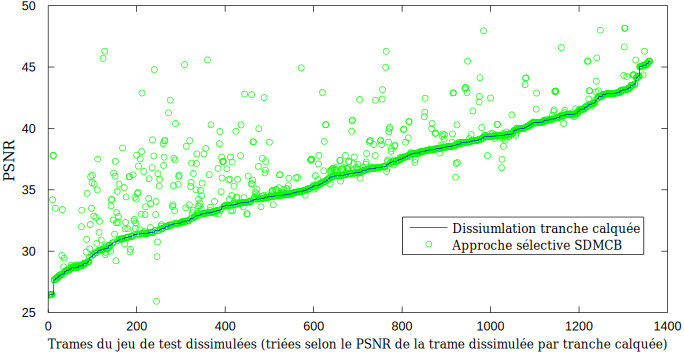
\includegraphics[width=\linewidth]{graphics/selectiveSliceCopy.pdf}\vspace{-1em}
\caption{\small{}Comparison of selective slice copy and the slice copy algorithms over
the 1360 sequences of our test dataset.}
\label{fig-SelectiveSliceCopy}
\end{figure*}

Enabling the decoder to select between slice copy and the erroneous slice is the
basis of our proposed selective slice copy approach. With $\textrm{SDMCB}$ as
our discriminant, we achieved the results shown in
Fig.~\ref{fig-SelectiveSliceCopy}. Selective slice copy produced an average gain
of 0.72~dB. In contrast, a reference-based selective algorithm (i.e. \DIFdelbegin \DIFdel{an ideal, 
but impossible to realize, method }\DIFdelend \DIFaddbegin \DIFadd{one }\DIFaddend that
selects the highest PSNR value between a frame copy and the erroneous frame when
compared against $\ltF{0}$) produced an optimal result of 0.94~dB. 

We observed that selective slice concealment makes an optimal choice in
82\% of the cases\DIFdelbegin \DIFdel{(compared to the reference-based method)}\DIFdelend . This allows the selective decoder to outperform the
conventional decoder in 32\% of cases, for an average gain of 1.95~dB.
In contrast, the reference-based selective algorithm produced an optimal gain of
2.12~dB.

The histogram in Fig.~\ref{fig-FrameDistribution} indicates that selective slice
concealment results in fewer poor concealments (\mbox{$<30$}~dB) and a larger
number of frames for every interval over 35~dB. This means that not only
does the proposed approach \DIFdelbegin \DIFdel{reduce }\DIFdelend \DIFaddbegin \DIFadd{reduces }\DIFaddend the number of low-quality concealments, these
having greater impact on the quality of the user experience, it also offers 
\DIFdelbegin \DIFdel{a
}\DIFdelend higher quality concealment without requiring additional bandwidth or a 
high-complexity algorithm.

Furthermore, $\textrm{SDMCB}$'s ability to choose the \DIFdelbegin \DIFdel{favorable }\DIFdelend \DIFaddbegin \DIFadd{favourable }\DIFaddend concealment 
could be exploited in future works for block level concealment such as \cite{OBMA}.
The advantages are twofold, by first identifying erroneous blocks that need
to be concealed (it has been shown that not all erroneous blocks require a concealment),
and \DIFdelbegin \DIFdel{second }\DIFdelend by offering a referenceless validation mechanism for concealment candidates \DIFdelbegin \DIFdel{,
}\DIFdelend as some
erroneous blocks will exhibit very little visual degradation.
\DIFaddbegin 

\begin{figure}%DIF > [htb]
\centering
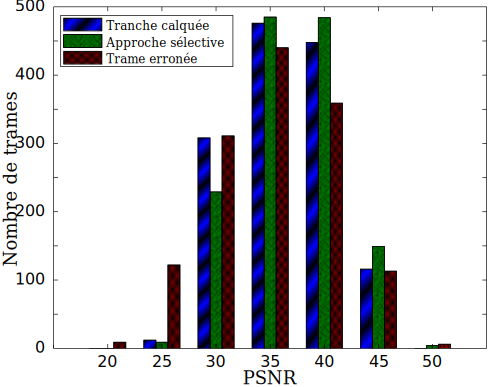
\includegraphics[width=1\linewidth]{graphics/FrameDistribution.pdf}\vspace{-1em}
\caption{\small{}\DIFaddFL{Frame PSNR histogram, with intervals of 5~dB centered at every 
5 dB increment after 20 dB, for 1360 erroneous frame concealments.}}
\label{fig-FrameDistribution}
\end{figure}
\DIFaddend \end{section}

%%%%%%%%%%%%%%%%%%%%%%%%%%%%%%%%% CONCLUSION %%%%%%%%%%%%%%%%%%%%%%%%%%%%%%%%%
\vspace{-0.5em}\begin{section}{Conclusion}
\DIFdelbegin %DIFDELCMD < \vspace{-0.5em}
%DIFDELCMD < %%%
\DIFdelend \label{section-conclusion}
In this paper, we described a novel visual degradation detection approach based
on the sum of distributed motion-compensated blockiness, $\textrm{SDMCB}$. We
proposed using this information for a low-complexity decoder \DIFdelbegin \DIFdel{add-on
}\DIFdelend \DIFaddbegin \DIFadd{postprocessing
}\DIFaddend operation that allows the \DIFdelbegin \DIFdel{decoder }\DIFdelend \DIFaddbegin \DIFadd{player }\DIFaddend to decide whether to use the erroneous slice or
slice copy. Our simulations show interesting ratios of decodable sequences based
on varying quantization parameters and bit error rates, and improved
concealment results when $\textrm{SDMCB}$ is used to guide the decoder in 
selecting between the erroneous slice and applying frame copy.  
These results constitute interesting avenues for decoders, players, and
no-reference video quality analysis tool makers.
\end{section}

\DIFdelbegin %DIFDELCMD < \begin{figure}
%DIFDELCMD < \centering
%DIFDELCMD < 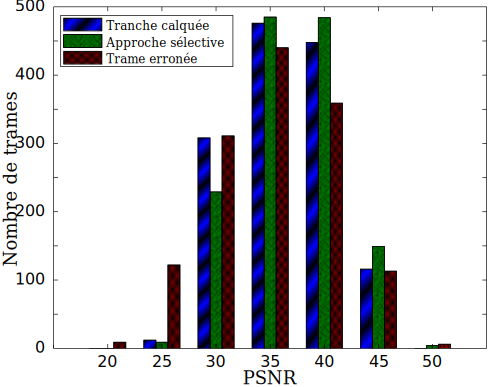
\includegraphics[width=1\linewidth]{graphics/FrameDistribution.pdf}\vspace{-1em}
%DIFDELCMD < %%%
%DIFDELCMD < \caption{%
{%DIFAUXCMD
%DIFDELCMD < \small{}%%%
\DIFdel{Frame PSNR histogram, with intervals of 5~dB centered at every 
5 dB increment after 20 dB, for 1360 erroneous frame concealments.}}
%DIFAUXCMD
%DIFDELCMD < \label{fig-FrameDistribution}
%DIFDELCMD < \end{figure}
%DIFDELCMD < 

%DIFDELCMD < \vspace{-0.75em}
%DIFDELCMD < \begin{spacing}{0.8} %%%
\DIFdelend \DIFaddbegin \vspace{-0.5em}
\begin{spacing}{0.9} \DIFaddend % tweak to fit
%DIF < \footnotesize % if needed, to fit
\DIFaddbegin \small %DIF >  if needed, to fit
\DIFaddend \bibliographystyle{IEEEbib}
\bibliography{article}
\end{spacing}
 \DIFdelbegin %DIFDELCMD < 

%DIFDELCMD <  %%%
\DIFdelend\end{document}
